\documentclass[11pt,a4paper]{article}

% ---------- Packages ----------
\usepackage[a4paper,margin=1in]{geometry}
\usepackage[utf8]{inputenc}
\usepackage[T1]{fontenc}
\usepackage{times}
\usepackage{graphicx}
\usepackage{booktabs}
\usepackage{array}
\usepackage{longtable}
\usepackage{caption}
\usepackage{enumitem}
\usepackage{titlesec}
\usepackage{fancyhdr}
\usepackage{xcolor}
\usepackage[colorlinks=true, linkcolor=blue, citecolor=blue, urlcolor=blue, breaklinks=true]{hyperref}
\usepackage{parskip}
\usepackage{tabularx}
\usepackage{ragged2e}
\usepackage{url}

% ---------- Page style ----------
\pagestyle{fancy}
\setlength{\headheight}{14pt}
\fancyhf{}
\renewcommand{\headrulewidth}{0.4pt}
\fancyhead[L]{E Commerce Order Experience Analysis}
\fancyhead[R]{Team 001}
\fancyfoot[C]{\thepage}

\setlength{\parindent}{0pt}

% ---------- Title spacing ----------
\titlespacing{\section}{0pt}{18pt}{8pt}
\titlespacing{\subsection}{0pt}{14pt}{6pt}

\newcolumntype{L}[1]{>{\RaggedRight\hspace{0pt}}p{#1}}

\begin{document}

% =========================================================
% TITLE PAGE
% =========================================================
\begin{titlepage}
    \centering
    \vspace*{1cm}
    
\includegraphics[width=3.2cm]{figs/iitm_logo.png}\par
    \vspace{1.2cm}

    {\Huge\bfseries E Commerce Order Experience Analysis\par}
    \vspace{0.6cm}
    {\Large Final Technical Report\par}
    \vspace{0.3cm}
    {\large Data Visualization Design Project\par}
    \vspace{0.3cm}
    {\large Marketplace Customer Satisfaction and Fulfilment Performance\par}

    \vspace{2cm}
    {\large 9th September 2026\par}

    \vfill

    {\large
    IITM BS Degree Program\\
    Indian Institute of Technology, Madras\\
    Chennai, Tamil Nadu, India, 600036\par}

    \vspace{1cm}
\end{titlepage}

\tableofcontents
\newpage

% =========================================================
\section*{Executive summary}
\addcontentsline{toc}{section}{Executive summary}

The marketplace can grow its seller base and order volume only if the post-purchase experience remains reliable. This report examines whether low customer ratings are mainly associated with the sellers and products admitted to the marketplace, or with fulfilment after checkout. The evidence points to delivery execution as the priority: late orders average 2.27 stars compared with 4.23 for on-time orders, and ratings fall to 2.61 stars when delivery takes 25 days or more.

The analysis uses a protected one-row-per-order dataset built from the Olist relational files. It follows the order journey from purchase to approval, seller handoff, carrier transit, delivery and review. The strongest actionable pattern is carrier transit, not seller handling: the average carrier stage is 8.9 days versus 2.3 days for seller handling, and satisfaction declines more steeply as carrier transit increases. Multi-seller orders are a second material source of dissatisfaction, while regional route conditions and a small group of high-value, low-scoring sellers identify where interventions should be targeted.

Management should protect growth by reducing the long delivery tail rather than applying broad seller restrictions. The immediate operating plan is to trigger delivery exceptions from day 16, set realistic region-specific carrier SLAs, disclose split fulfilment at checkout, and provide dedicated remediation to the most commercially important at-risk sellers.

\newpage

% =========================================================
\section{Business problem and decision questions}

\subsection{Business problem in our words}
The marketplace wants more sellers and more sales, but cannot allow expansion to reduce customer satisfaction. Management needs to know which parts of the order journey create low reviews, whether these problems can be fixed operationally, and how to intervene without unnecessarily reducing seller participation or commercial volume.

\subsection{Questions the analysis answers}
\begin{itemize}[leftmargin=1.2cm]
    \item How strongly do delivery duration and late delivery affect review scores?
    \item Is the satisfaction loss more closely associated with seller handling or carrier transit?
    \item Do multi-seller orders create a separate fulfilment-complexity penalty?
    \item Which regions, routes and sellers should receive priority intervention?
    \item Do categories, price, payment, freight and geography alter the conclusion that fulfilment is the main operational lever?
\end{itemize}

% =========================================================
\section{Analytical approach and design rationale}

We treated the customer review as the final outcome of an order journey rather than as an isolated seller score. The analytical sequence was: understand the relational data, create a reliable order-level dataset, measure the core delivery outcomes, test plausible alternative explanations, and translate the evidence into a dashboard and operating actions. This design prevents the project from becoming a collection of unrelated charts.

\subsection{Analytical logic}
The primary hypothesis was that slower or late fulfilment lowers satisfaction. We then split the delivery journey into approval, seller handling and carrier transit to locate the responsible stage. We tested multi-seller fulfilment, geography, category, freight, payment and product characteristics as competing explanations. This is descriptive exploratory analysis, not a causal experiment; the findings are therefore used to prioritise operational investigation and intervention testing.

\begin{table}[h]
\centering
\caption{Analytical framework}
\begin{tabularx}{\textwidth}{L{2.6cm} L{5.6cm} L{5.6cm}}
\toprule
\textbf{Phase} & \textbf{Purpose} & \textbf{Business value} \\
\midrule
Understand & Map source-table grain and define one order as the unit of analysis. & Ensures each customer experience receives one fair vote. \\
Prepare & Aggregate one-to-many tables before joining and derive fulfilment metrics. & Prevents duplicate reviews and creates comparable measures. \\
Explore & Compare ratings across delivery, delay, seller, region and order-structure segments. & Identifies where dissatisfaction is concentrated. \\
Communicate & Use decision-oriented charts and an interactive dashboard. & Makes owner, priority and action clear to management. \\
\bottomrule
\end{tabularx}
\end{table}

% =========================================================
\section{Data preparation and quality assurance}

\subsection{Source data and analytical grain}
The source is a relational marketplace dataset. Orders, items, payments and reviews do not have the same grain: one order can contain several items, payment records and review entries. The analytical dataset was deliberately built at one row per order because both delivery outcome and review score are experienced at order level.

\begin{table}[h]
\centering
\caption{Source tables and preparation rules}
\begin{tabularx}{\textwidth}{L{3.2cm} L{4.8cm} L{5.8cm}}
\toprule
\textbf{Source group} & \textbf{Role in analysis} & \textbf{Preparation rule} \\
\midrule
Orders & Order status and lifecycle timestamps. & Used as the order-level spine. \\
Items and products & Item count, seller count, category, price and freight. & Aggregated by order before joining. \\
Payments & Payment value, type and instalments. & Total payment summed; method retained as a descriptor. \\
Reviews & Review score and comment availability. & Duplicate reviews averaged by order. \\
Customers, sellers and geolocation & Customer state, seller state and route context. & Joined after grain-safe aggregation. \\
\bottomrule
\end{tabularx}
\end{table}

\subsection{Cleaning and aggregation decisions}
\begin{itemize}[leftmargin=1.2cm]
    \item Standardised identifiers, numeric fields and timestamps before any calculation.
    \item Excluded orders without item rows from fulfilment comparisons because seller and delivery measures cannot be meaningfully defined for them. This explains the difference between 99,441 raw orders and 98,666 master-order rows.
    \item Averaged the 551 duplicated review records by order ID, preventing one order from receiving multiple votes in rating summaries.
    \item Summed payment values and aggregated payment characteristics before joining, avoiding row multiplication from split payments.
    \item Retained unusually long deliveries after validating the underlying timestamps; these are business-relevant service failures, not automatic data errors.
    \item Flagged missing or logically impossible time intervals rather than interpreting them as operational performance.
\end{itemize}

\subsection{Derived variables and why they matter}

\begin{table}[h]
\centering
\caption{Derived measures}
\begin{tabularx}{\textwidth}{L{2.8cm} L{5.4cm} L{5.6cm}}
\toprule
\textbf{Derived measure} & \textbf{Definition} & \textbf{Decision supported} \\
\midrule
Delivery time & Customer delivery date minus purchase timestamp. & Identifies the satisfaction threshold. \\
Late delivery & Actual delivery later than estimated delivery date. & Measures promise reliability. \\
Seller handling & Carrier handoff minus approval date. & Separates merchant-stage delay. \\
Carrier transit & Customer delivery minus carrier handoff. & Separates transport-stage delay. \\
Distinct sellers & Number of sellers represented in an order. & Measures split-fulfilment complexity. \\
Seller risk & Seller-level order-value proxy, average score and late rate. & Targets high-value remediation. \\
\bottomrule
\end{tabularx}
\end{table}

% =========================================================
\section{Findings and visual evidence}

\subsection{Delivery time is the dominant satisfaction signal}
Delivery duration has a clear non-linear relationship with satisfaction. Ratings remain above four stars through 15 days, worsen after 16 days, and collapse in the 25+ day group. The business implication is to prevent the extreme tail, not to spend resources shaving small increments from already fast deliveries.

\begin{figure}[h]
\centering
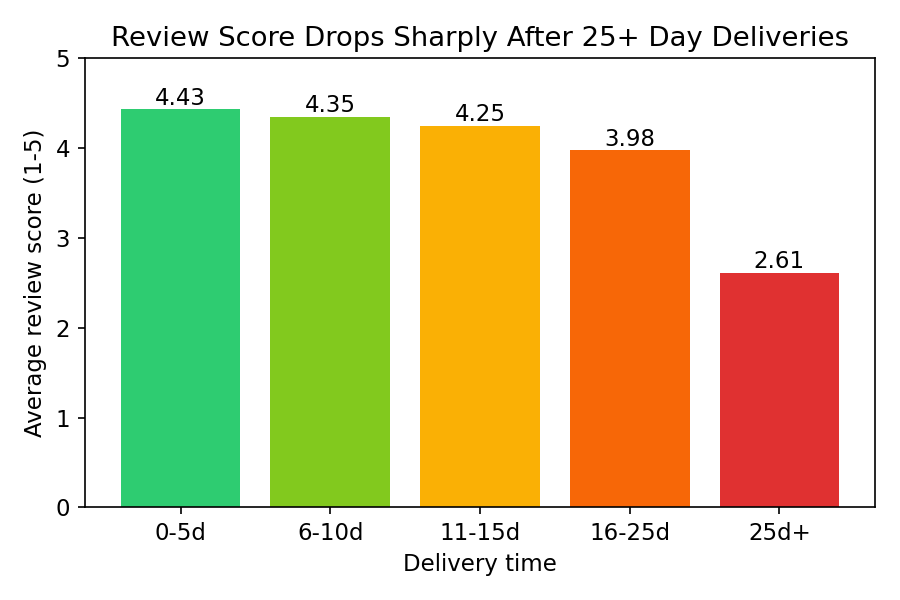
\includegraphics[width=0.75\textwidth]{figs/fig1_delivery_bucket.png}
\caption{Average review score and one-star share by delivery-time bucket. Orders delivered in 25+ days average 2.61 stars and have a 43.6\% one-star share, compared with high ratings in the 0--15 day bands.}
\end{figure}

\begin{figure}[h]
\centering
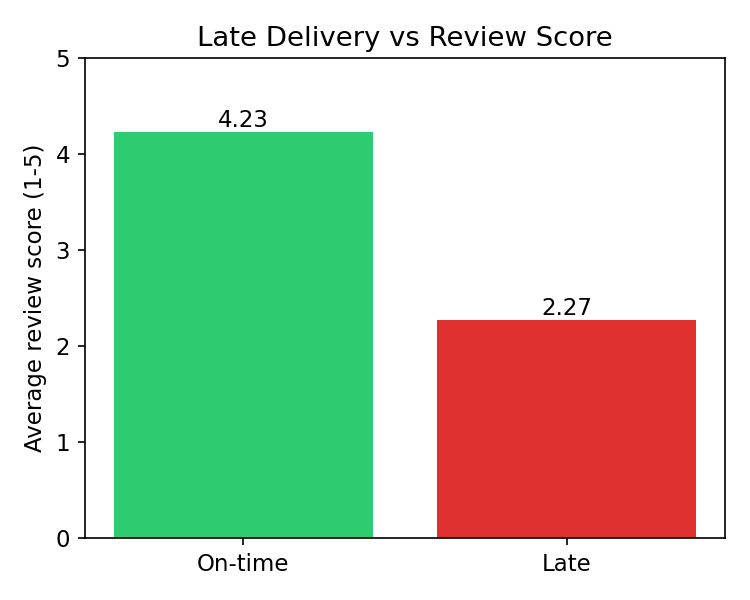
\includegraphics[width=0.7\textwidth]{figs/fig2_late_delivery.png}
\caption{Late delivery versus review score. On-time orders average 4.23 stars; late orders average 2.27. The 1.96-star gap makes promise reliability a central management KPI.}
\end{figure}

\subsection{Carrier transit is the primary operational bottleneck}
Decomposing the fulfilment journey avoids blaming sellers for delays that occur after carrier handoff. Carrier transit shows a stronger negative association with review score than seller handling. Its average duration is 8.9 days, compared with 2.3 days for seller handling, and satisfaction degrades more sharply as transit length increases.

\begin{figure}[h]
\centering
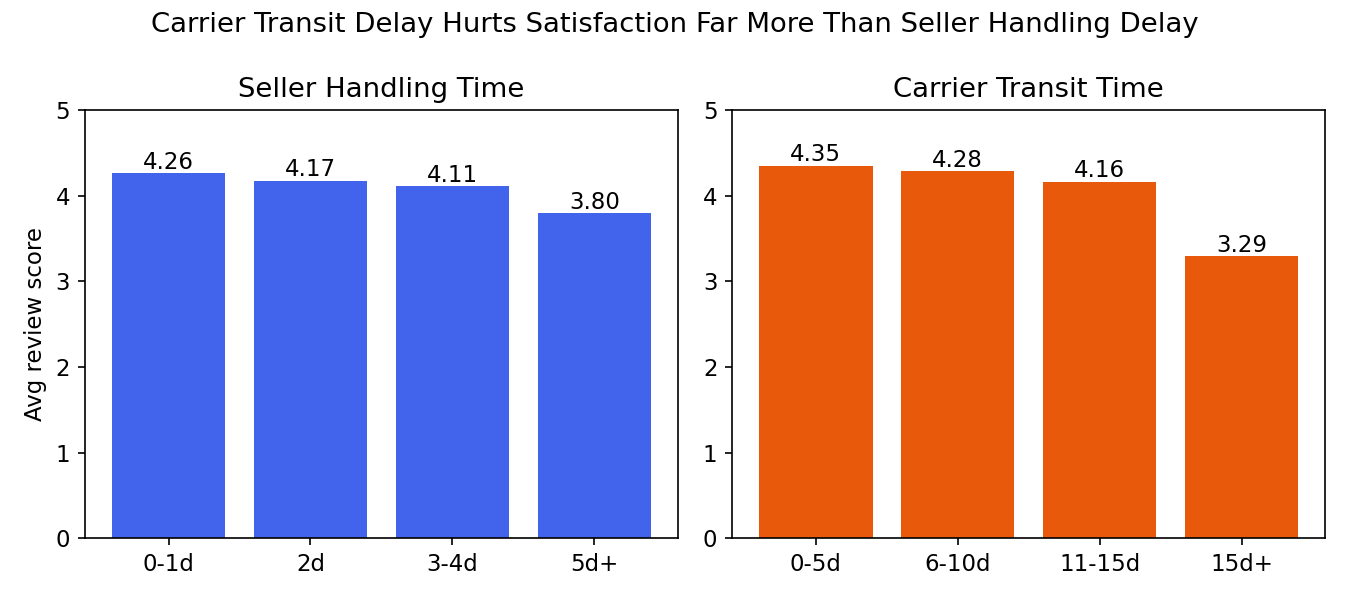
\includegraphics[width=0.85\textwidth]{figs/fig3_seller_carrier.png}
\caption{Seller handling and carrier transit delay versus review score. The sharper carrier-transit decline assigns the first operational owner to carrier routing, handoffs and exception management.}
\end{figure}

\subsection{Split fulfilment creates a separate complexity penalty}
Order size alone is not the main issue. When an order is supplied by more than one seller, customers may receive several packages and experience fragmented tracking. One-seller orders average 4.12 stars, while two-seller orders drop to 2.88 stars; three and four-plus seller orders are lower still.

\begin{figure}[h]
\centering
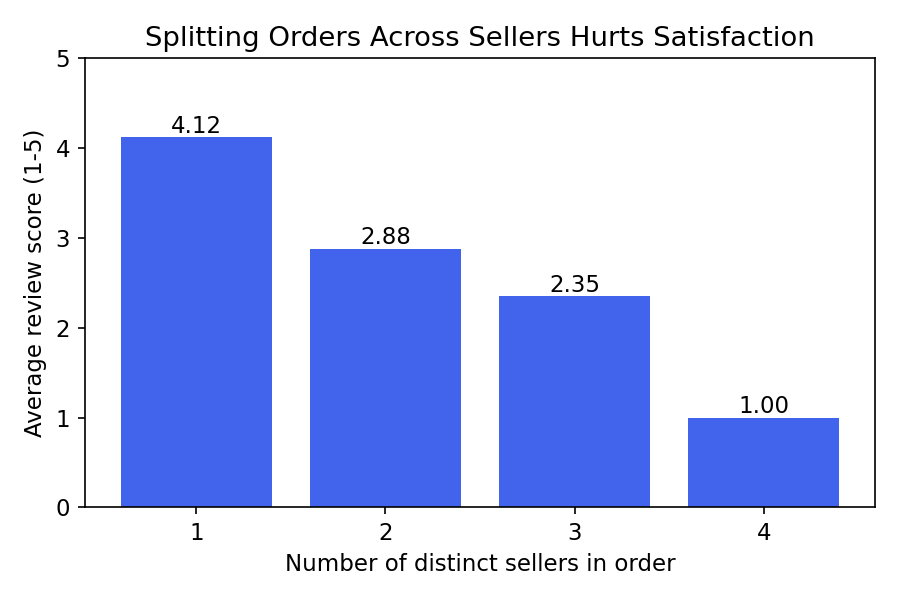
\includegraphics[width=0.7\textwidth]{figs/fig4_nsellers.png}
\caption{Average review score by distinct sellers in an order. The steep drop after the first seller supports checkout disclosure and split-package tracking rather than a generic restriction on multi-item baskets.}
\end{figure}

\subsection{Regional routes and commercial concentration define where to act}
Distance is associated with longer delivery time, and the dashboard shows that Northern and Northeastern states experience the longest delivery durations and higher late-delivery rates. Regional SLAs should therefore reflect route realities. At seller level, revenue is concentrated: the top 1\% of sellers account for 26.1\% of order value and the top 10\% account for 67.5\%. A small number of high-value, low-scoring sellers can therefore create material satisfaction and commercial risk.

\begin{figure}[h]
\centering
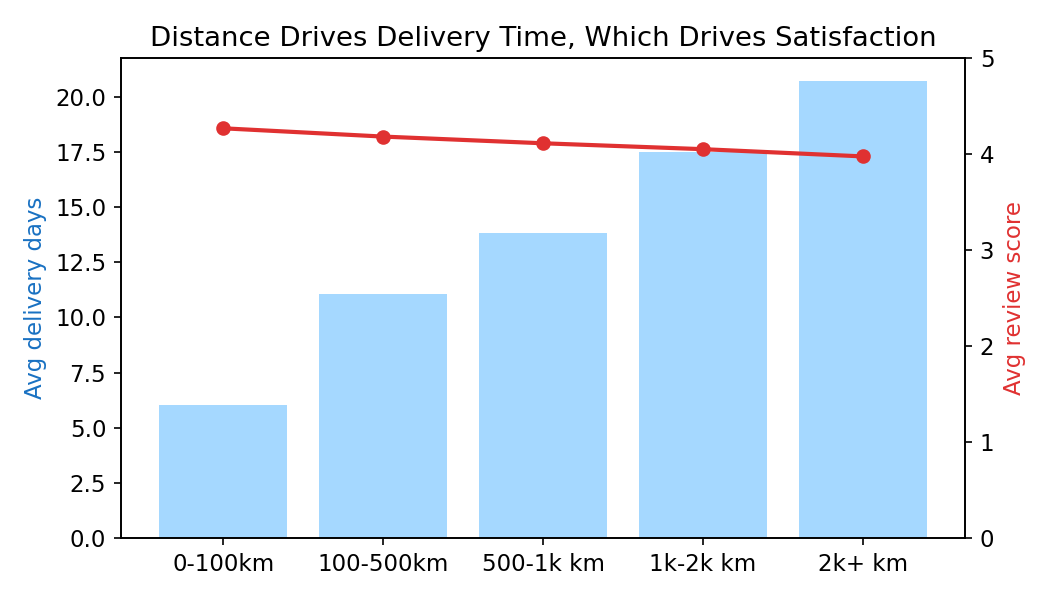
\includegraphics[width=0.8\textwidth]{figs/fig5_distance.png}
\caption{Distance, delivery time and review score. Distance matters mainly because it lengthens the delivery journey; it is not itself the direct management lever.}
\end{figure}

\begin{figure}[h]
\centering
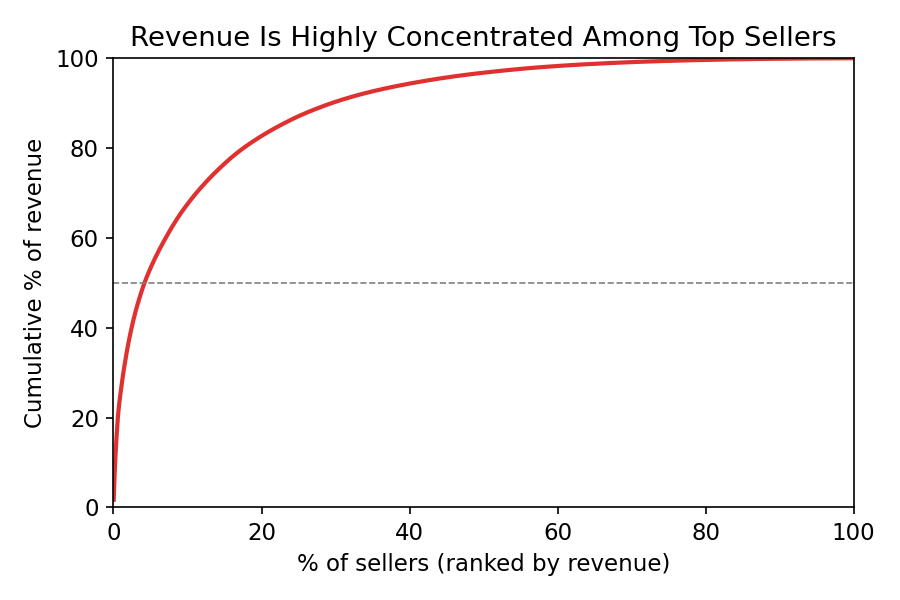
\includegraphics[width=0.75\textwidth]{figs/fig6_revenue_concentration.png}
\caption{Cumulative seller revenue concentration. Commercial concentration supports targeted support for high-value at-risk sellers rather than blanket seller bans.}
\end{figure}

\subsection{Alternative explanations were examined, but do not overturn the conclusion}
Product category, price, freight, payment type, instalments and same-state delivery were examined to avoid assuming that logistics was the answer. Some categories have lower ratings, and same-state orders are faster and slightly better rated, but these differences are materially smaller than the late-delivery and 25+ day effects. Category evidence is therefore useful for monitoring but not the first operating priority.

\begin{figure}[h]
\centering
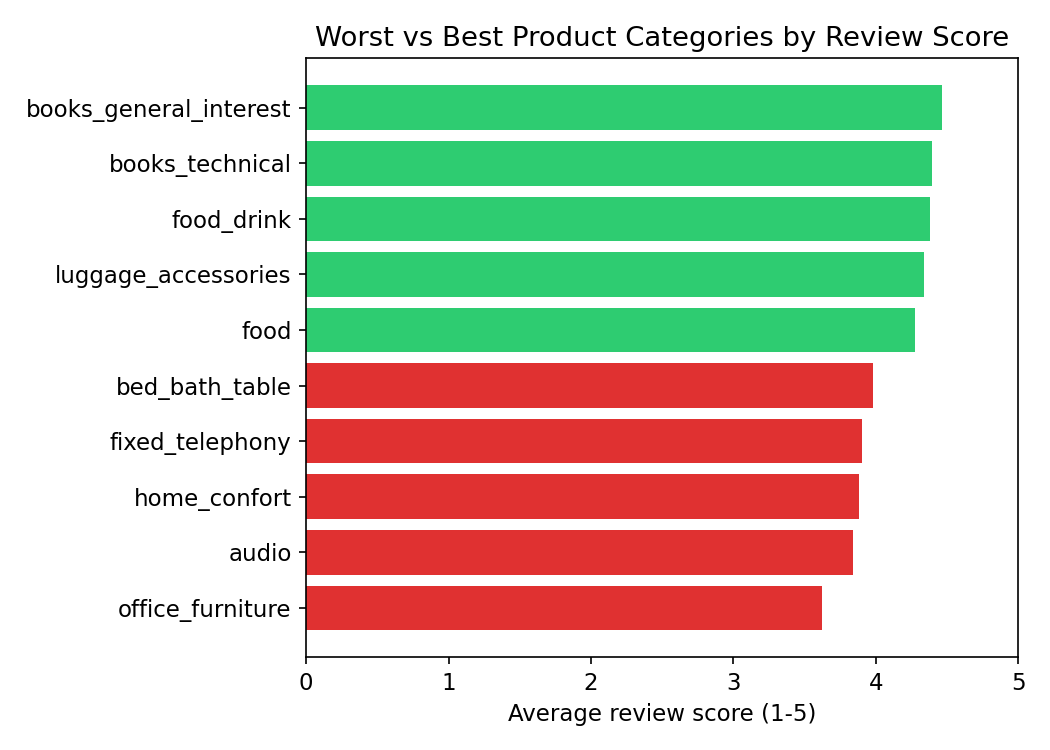
\includegraphics[width=0.85\textwidth]{figs/fig7_categories.png}
\caption{Best and worst product categories by average review score. Category differences exist, but they are secondary to the large delivery and lateness gaps.}
\end{figure}

% =========================================================
\section{Dashboard design and chart selection}

The dashboard was designed for management action, not for displaying every available variable. Each visual answers one decision question and connects to a named operational response. The published dashboard is available in the appendix.

\begin{table}[h]
\centering
\caption{Dashboard visual selection rationale}
\begin{tabularx}{\textwidth}{L{3.0cm} L{5.0cm} L{5.0cm}}
\toprule
\textbf{Dashboard visual} & \textbf{Why this chart type} & \textbf{Decision it supports} \\
\midrule
Satisfaction cliff & Grouped bars show rating and one-star share by delivery band. & Prioritise the 25+ day tail. \\
Seller versus carrier & Grouped bars compare two fulfilment stages across delay bands. & Assign ownership to carrier operations. \\
Seller risk quadrant & Scatter plot reveals revenue-score trade-offs and outliers. & Target high-value low-score sellers. \\
Logistics complexity & Bar chart makes the seller-count penalty immediately visible. & Improve split-order communication. \\
Regional performance & Sorted dual-metric view compares delivery time and late rate by state. & Set route-specific SLA policy. \\
Complaint themes & Treemap summarises tagged review-comment themes. & Use qualitative context for service recovery. \\
\bottomrule
\end{tabularx}
\end{table}

% =========================================================
\section{Management implications and recommendations}

\subsection{Prioritised action plan}

\begin{table}[h]
\centering
\caption{Prioritised action plan}
\begin{tabularx}{\textwidth}{c L{4.0cm} L{4.0cm} L{4.2cm}}
\toprule
\textbf{Priority} & \textbf{Action} & \textbf{Evidence} & \textbf{Owner and KPI} \\
\midrule
1 & Trigger carrier exceptions at day 16 and prevent orders reaching 25+ days. & Ratings collapse to 2.61 stars in the 25+ day band. & Carrier operations; 25+ day share and late rate. \\
2 & Use regional service promises and carrier SLAs for long-distance routes. & Long delivery and high late rates cluster in remote regions. & Logistics planning; state-level delivery days and late rate. \\
3 & Show split-delivery expectations and tracking at checkout. & Two-seller orders average 2.88 versus 4.12 for one seller. & Marketplace product; multi-seller rating gap. \\
4 & Give high-value at-risk sellers dedicated logistics support and review monitoring. & Top 10\% sellers account for 67.5\% of order value. & Merchant partnerships; seller late rate and score. \\
5 & Use category and complaint themes for diagnosis after fulfilment actions are underway. & Secondary patterns do not explain the main satisfaction cliff. & Customer experience; issue-theme trend. \\
\bottomrule
\end{tabularx}
\end{table}

\subsection{Recommended operating cadence}
\begin{itemize}[leftmargin=1.2cm]
    \item \textbf{Daily}: flag carrier-transit exceptions approaching day 16 and trigger proactive customer communication.
    \item \textbf{Weekly}: review late rate, 25+ day share, split-order rating gap and regional SLA performance.
    \item \textbf{Monthly}: review the high-value seller risk quadrant and agree joint carrier-seller remediation actions.
    \item \textbf{Quarterly}: evaluate whether interventions improve satisfaction while maintaining seller growth and order volume.
\end{itemize}

\subsection{Leadership decisions}
Leadership should treat delivery reliability as a growth guardrail, not as a back-office logistics metric. The commercial objective is not simply to reduce average delivery time; it is to stop the small but damaging tail of orders that cross into the 25+ day experience. That tail produces disproportionately low ratings and visible complaint risk, so it should be managed as an exception portfolio with clear executive ownership.

\begin{itemize}[leftmargin=1.2cm]
    \item Set one executive outcome: reduce the 25+ day share and late-delivery rate while holding seller growth and order volume steady. This prevents operational improvement from being pursued at the expense of marketplace expansion.
    \item Make carrier performance a commercial governance issue. Route-level SLAs, escalation thresholds and carrier scorecards should be reviewed with the same discipline as seller performance because carrier transit is the strongest satisfaction bottleneck.
    \item Avoid blanket seller penalties. The top 10\% of sellers represent 67.5\% of order value, so indiscriminate removal of low-scoring sellers risks revenue. Use the risk quadrant to concentrate account management and logistics support where both satisfaction and commercial exposure are high.
    \item Design for customer expectation, not only physical speed. For multi-seller carts, accurate split-package dates, proactive notifications and parcel-level tracking can reduce perceived failure even where multiple deliveries remain necessary.
    \item Fund a fulfilment control tower. A recurring view of transit exceptions, regional SLA gaps, high-value seller risk and complaint themes will let leadership see emerging risk before it becomes a review-score problem.
\end{itemize}

\subsection{Leadership scorecard and decision gates}
Leadership should not use average delivery time alone as the success measure. An average can improve while a small set of customers still experience the 25+ day service failure that causes the most damage. The scorecard should therefore combine customer outcome, operational reliability and commercial protection. Each monthly review should decide whether to scale an intervention, redesign it, or stop it based on these measures.

\begin{table}[h]
\centering
\caption{Leadership scorecard and decision gates}
\begin{tabularx}{\textwidth}{L{3.4cm} L{4.8cm} L{4.8cm}}
\toprule
\textbf{Leadership measure} & \textbf{Why it matters} & \textbf{Decision gate} \\
\midrule
25+ day delivery share & Directly monitors the satisfaction cliff, where average rating falls to 2.61. & Escalate routes or carriers that do not reduce the tail after intervention. \\
Late-delivery rate & Measures whether the platform keeps its customer promise. & Hold carrier and route owners accountable to agreed SLA targets. \\
On-time versus late rating gap & Confirms whether reliability is still translating into customer experience. & Investigate if the gap persists after service recovery changes. \\
Multi-seller rating gap & Shows whether checkout communication reduces split-fulfilment friction. & Scale parcel-level tracking if the gap narrows without lower conversion. \\
Seller growth and order volume & Prevents quality actions from harming marketplace expansion. & Do not deploy blanket seller restrictions if growth is put at risk. \\
High-value seller risk count & Tracks the number of commercially material sellers below the platform score benchmark. & Target account and logistics support before punitive action. \\
\bottomrule
\end{tabularx}
\end{table}

\subsection{Recommended 90 day leadership roadmap}

\begin{table}[h]
\centering
\caption{90 day leadership roadmap}
\begin{tabularx}{\textwidth}{L{2.4cm} L{5.0cm} L{5.0cm}}
\toprule
\textbf{Timing} & \textbf{Leadership commitment} & \textbf{Expected learning} \\
\midrule
Days 0--30 & Nominate a fulfilment owner, publish the route and carrier scorecard, and activate day-16 exception alerts. & Which carriers and routes generate the avoidable long-tail orders. \\
Days 31--60 & Pilot regional SLA messages, proactive delay communication and parcel-level tracking for multi-seller orders. & Whether better expectation-setting narrows the review-score gap. \\
Days 61--90 & Review the seller risk quadrant with merchant partnerships and scale the best-performing carrier and checkout interventions. & Which actions improve satisfaction without slowing seller and order growth. \\
\bottomrule
\end{tabularx}
\end{table}

% =========================================================
\section{Constraints and next steps}

This report is descriptive. Timing associations identify where to investigate and intervene, but do not prove that every low score was caused by the measured delay. Payment value is recorded at order level, so seller-level revenue is an analytical allocation proxy in multi-seller orders. Review comments are self-selected and any tagged complaint themes should be documented with the exact Portuguese keyword and classification rules. Future work should test interventions with before-after or controlled comparisons, add carrier-level identifiers where available, and monitor results over time.

\newpage
% =========================================================
\section*{Technical appendix}
\addcontentsline{toc}{section}{Technical appendix}

\subsection*{A. Data preparation pseudocode}
\addcontentsline{toc}{subsection}{A. Data preparation pseudocode}

\begin{verbatim}
LOAD orders, order_items, payments, reviews, customers, sellers,
     products and geography tables
STANDARDISE identifiers, numeric fields and timestamps; set one row
     per order_id as the target grain
AGGREGATE items by order_id: n_items, n_sellers, price, freight and
     category descriptors
AGGREGATE payments by order_id: total payment, payment method and
     maximum instalments
AGGREGATE reviews by order_id: mean review score and comment-
     availability indicator
JOIN aggregates to delivered orders; attach customer, seller, product
     and geographic attributes
DERIVE delivery time, late flag, seller handling, carrier transit,
     seller-count and delay buckets
VALIDATE duplicates, null rates, negative intervals, timestamp order
     and extreme delivery durations
GROUP BY required segment for charts; calculate average score, order
     count and late-delivery rate
PUBLISH grouped results to the dashboard and retain metric
     definitions beside each visual
\end{verbatim}

\subsection*{B. Metric definitions}
\addcontentsline{toc}{subsection}{B. Metric definitions}

\begin{table}[h]
\centering
\caption{Metric definitions}
\begin{tabularx}{\textwidth}{L{4.0cm} L{9.5cm}}
\toprule
\textbf{Metric} & \textbf{Formula or rule} \\
\midrule
Average review score & Mean review score at the aggregated order level. \\
Delivery time & delivered\_customer\_date minus purchase\_timestamp in days. \\
Late delivery & delivered\_customer\_date later than estimated\_delivery\_date. \\
Seller handling & carrier\_handoff\_date minus approved\_date. \\
Carrier transit & delivered\_customer\_date minus carrier\_handoff\_date. \\
Late-delivery rate & late delivered orders divided by delivered orders in the segment. \\
\bottomrule
\end{tabularx}
\end{table}

\subsection*{C. Project artefacts and evaluator links}
\addcontentsline{toc}{subsection}{C. Project artefacts and evaluator links}

All artefacts required to review, reproduce and audit this analysis are listed below. Every link has been checked for evaluator accessibility prior to submission (last verified 9th September 2026).

\begin{table}[h]
\centering
\caption{Project artefacts and evaluator access links}
\begin{tabularx}{\textwidth}{L{3.6cm} L{9.9cm}}
\toprule
\textbf{Artefact} & \textbf{Link} \\
\midrule
Interactive executive dashboard &
\url{https://dvd-project-fawn.vercel.app} \\[4pt]
GitHub repository (code, notebooks, work logs) &
\url{https://github.com/blurrydev/IITM-DVD} \\[4pt]
Google Drive dataset folder (raw and enriched data, figures, supporting documents) &
\url{https://drive.google.com/drive/folders/1CZemi5Ws71fA9cniJ_gN4Kcjk8fP45F_?usp=drive_link} \\[4pt]
Mid-Week EDA Report (source on GitHub) &
\url{https://github.com/blurrydev/IITM-DVD/tree/main/report} on the GitHub repository above \\[4pt]
Final technical report (this document; source also on GitHub) &
\url{https://github.com/blurrydev/IITM-DVD/tree/main/report} on the GitHub repository above \\[4pt]
Final presentation &
\url{https://drive.google.com/drive/folders/1TaFyAda0lBb3GN_nzA3eKT3QZiAgSCsO?usp=sharing} \\
\bottomrule
\end{tabularx}
\end{table}

\textbf{Accessibility note.} The dashboard and GitHub links were confirmed reachable without authentication at the time of writing. The Google Drive folder must be set to ``Anyone with the link can view'' and re-tested in an incognito browser window before final submission, since Drive permissions can silently revert to restricted access. The Kaggle notebook and final presentation links are placeholders and must be completed before submission; an evaluator following this appendix cannot yet reach those two artefacts.

\subsection*{D. Tools and project artefact management}
\addcontentsline{toc}{subsection}{D. Tools and project artefact management}

\begin{table}[h]
\centering
\caption{Tools, platforms and their role in the project}
\begin{tabularx}{\textwidth}{L{3.6cm} L{5.0cm} L{4.9cm}}
\toprule
\textbf{Tool or platform} & \textbf{Use in the project} & \textbf{Submission role} \\
\midrule
Python scripts & Repeatable extraction, cleaning, aggregation, feature engineering, checks and chart-ready datasets. & Provides the reproducible analytical pipeline. \\
LaTeX and Overleaf & Final typesetting, structured citations, equations and submission-ready report compilation. & Provides an evaluator-ready PDF workflow and a controlled report source. \\
Microsoft Word & Collaborative drafting, review, editing and stakeholder-facing documentation. & Supports document development and formatting review before final submission. \\
GitHub & Version-controlled codebase, work logs, notebook history and dashboard source files. & Provides evaluator access to reproducible code and contribution history. \\
Google Drive & Shared source extracts, enriched dataset, figures and supporting project documents. & Provides controlled sharing of large data artefacts. \\
Browser based dashboard deployed on Vercel & Interactive management dashboard with decision-oriented visuals, filters and chart interactions. & Provides a live companion artefact for evaluators and leadership. \\
\bottomrule
\end{tabularx}
\end{table}

\end{document}
